\documentclass[a4paper,11pt]{article}
\usepackage[utf8]{inputenc}
\usepackage{minted}
\usepackage{amsmath}
\usepackage{float}
\usepackage[symbol]{footmisc}
\usepackage{graphicx}
\usepackage[toc,page]{appendix}

\graphicspath{{./figures/}}
\renewcommand{\thefootnote}{\fnsymbol{footnote}}

\title{\textbf{8. Queue}}
\author{Kristiāns Vinters}
\date{Fall 2023}

\begin{document}
    \maketitle
    \section*{Introduction}

    I solved the assignment in Go. I used Go because I want to become more familiar with it. Source code and benchmark data is available on GitHub\footnote[1]{https://github.com/Phanty133/id1021/tree/master/8-queue}.

    \section*{Implementation}

    There weren't any particular difficulties in implementing a queue in Go. For the linked list queue, I reused the linked list implementation from a previous assignment. To make benchmarking easier, I defined a common interface for all queue implementations.

    \begin{minted}{go}
type Queue[T comparable] interface {
    // Add an element to the queue, error if full (if static size)
    Enqueue(val T) error

    // Remove an element from the queue and return it, error if empty
    Dequeue() (T, error)

    // True if the queue is empty
    Empty() bool
}
    \end{minted}

    The linked list queue was very straightforward to implement by just using \texttt{ll.append()} to add elements to the queue and accessing and removing the first element to dequeue. An empty queue was defined as a queue with a \texttt{nil} first element.

    Both the static and dynamic array queues share a similar structure with the exception that the dynamic array also tracks the count of elements in the queue to know when to downsize.

    \begin{minted}{go}
type QueueStatic[T comparable] struct {
    data  []T
    front int
    back  int
}

type QueueDynamic[T comparable] struct {
    data  []T
    front int
    back  int
    count int
}
    \end{minted}

    The static and dynamic array queues share a function that handles index wrapping logic. The wrapping was implemented by incrementing the index modulo capacity of the array. A particularity of Go is that the built-in modulo \texttt{\%} operator has different conventions compared to modulo in math. Instead of always returning the least positive remainder, it returns the last absolute remainder. This means that \texttt{-1 \% 5} returns \texttt{-1} instead of \texttt{4}. To fix this, I implemented a custom modulo function that always returns the least positive remainder. 

    \begin{minted}{go}
func mod(a, b int) int {
    return (a%b + b) % b
}       

func (q *QueueStatic[T]) nextIndexWrapped(idx int) int {
    return mod((idx + 1), cap(q.data))
}
    \end{minted}

    Both implementations also shared the same logic for determining when the queue is full and empty. A queue was considered full when the back and front indices were equal and they pointed to a non-zero element, whereas it was considered empty when both were equal and pointed to a zero element.

\begin{minted}{go}
// Check for full from QueueStatic.go
if q.back == q.front && !q.Empty() {
    return errors.New("queue is full")
}

// Empty check from QueueStatic.go
func (q *QueueStatic[T]) Empty() bool {
    var zero T
    return q.back == q.front && q.data[q.front] == zero
}
\end{minted}

    The only difference between the static and dynamic implementation, of course, is that when enqueueing a new element, if the dynamic queue is full, it reallocates itself with a larger data array. When dequeueing, if the queue is less than a quarter full, it reallocates itself with a smaller data array. When reallocating, I reorganize the queue such that the front is always at index 0. I handle the data copying for upsizing and downsizing differently. If upsizing, it means that the entire queue is full and so I copy all elements from the front to the end of the current array to the new array starting at 0 and then copy the remaining elements from the start of the current array to the end of the new array. If downsizing, it means that the queue is less than a quarter full and so I copy all elements from the front to the end of the current array to the new array starting at 0.

    \begin{minted}{go}
func (q *QueueDynamic[T]) Reallocate(newSize int) {
    newData := make([]T, newSize)

    if newSize < cap(q.data) {
        copy(newData, q.data[q.front:q.front+q.count])
    } else {
        endDist := cap(q.data) - q.front
        copy(newData[0:endDist], q.data[q.front:])
        copy(newData[endDist:], q.data[:q.front])
    }

    q.front = 0
    q.back = q.count
    q.data = newData
}
    \end{minted}

    The \texttt{Reallocate} function is called from the \texttt{Enqueue} and \texttt{Dequeue} functions.

    \begin{minted}{go}
func (q *QueueDynamic[T]) Enqueue(val T) error {
    if q.back == q.front && !q.Empty() {
        q.Reallocate(cap(q.data) * 2)
    }
    // ...
    q.count++
    // ...
}

func (q *QueueDynamic[T]) Dequeue() (T, error) {
    // ...
    q.count--

    if q.count < cap(q.data)/4 {
        q.Reallocate(cap(q.data) / 2)
    }

    // ...
}
    \end{minted}

    \section*{Benchmarking}

    I benchmarked the queues by running them 500 times on different, randomly generated integer arrays for array sizes 10, 100, 1000, 5000, 10000, 50000, 100000, 500000, 1000000. I performed two benchmarks - 1. Allocation+Enqueuing N elements; 2. Dequeueing N elements. I chose to measure allocation and enqueueing together because otherwise the static array queue would have an unfair advantage over the others, as it'd be entirely preallocated. I also figured that allocation+enqueue is a realistic use case for queues. I also ran two benchmarks for the linked list queue - one with a standard singly-linked list and one for a linked list that tracks the pointer of the last element. For analyzing run times, I measured the raw execution time for every repeat in nanoseconds, which I stored in an array and then wrote to a \texttt{.csv} file. I used LibreOffice Calc to calculate the mean, median, min, and max times and plot the graphs.

    For the allocation+enqueue benchmark, the static and dynamic queue times were similar, however the static queue was generally more performant. The linked list with the last pointer had an approximately 3-3.5x times worse performance on average (fig. \ref{fig:ae-table}). These three structures have the same time complexity, whereas the linked list without a last pointer had a higher complexity, as well as a much higher runtime for all N (fig. \ref{fig:ae}). This is because the linked list has to traverse the entire list every time a new element needs to be enqueued.

    \begin{figure}[H]
        \centering
        
        \begin{tabular}{c|c|c|c|c}
            Size & $t_\text{Static}$, $\mu s$ & $t_\text{Dynamic}$, $\mu s$ & $t_\text{LL, last ptr}$, $\mu s$ & $t_\text{LL, std}$, $\mu s$ \\
            \hline
            \hline
            100 & 1.89 & 1.89 & 3.28 & 8.42 \\
            \hline
            1000 & 6.71 & 8.10 & 23.4 & 522 \\
            \hline
            5000 & 30.0 & 36.3 & 113 & 12500 \\
            \hline
            10000 & 57.8 & 69.0 & 228 & 48100 \\
            \hline
            50000 & 436 & 308 & 1110 & 1220000 \\
            \hline
            100000 & 554 & 749 & 2215 & 4880000 \\
            \hline
            500000 & 3170 & 3990 & 14100 & DNF \\
            \hline
            1000000 & 6070 & 7840 & 27700 & DNF \\
        \end{tabular}

        \caption{Allocation+Enqueue benchmark median times}
        \label{fig:ae-table}
    \end{figure}

    \begin{figure}[H]
        \centering
        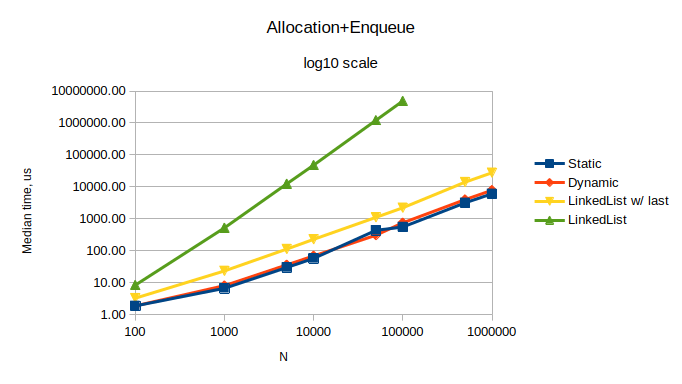
\includegraphics[width=\textwidth]{ae.png}
        \caption{Median allocation+enqueue times}
        \label{fig:ae}
    \end{figure}

    For the dequeueing benchmark, the runtimes for all implementations were much more similar (fig. \ref{fig:d-table}). All of the implementations had the same complexity (fig. \ref{fig:d}). The static and dynamic array queues still had similar performance, however in this benchmark both linked lists generally performed better than the arrays. Both linked list implementations had very similar performance because when dequeueing, the last element does not need to be accessed. I suspect that the linked lists outperformed the arrays in this benchmark because it's much quicker to move pointers around instead of having to perform a modulo operation for the index and doing extra checks for a full array.

    \begin{figure}[H]
        \centering
        
        \begin{tabular}{c|c|c|c|c}
            Size & $t_\text{Static}$, $\mu s$ & $t_\text{Dynamic}$, $\mu s$ & $t_\text{LL, last ptr}$, $\mu s$ & $t_\text{LL, std}$, $\mu s$ \\
            \hline
            \hline
            100 & 1.82 & 1.89 & 1.47 & 1.40 \\
            \hline
            1000 & 6.64 & 7.12 & 4.19 & 4.26 \\
            \hline
            5000 & 28.6 & 33.2 & 18.5 & 16.13 \\
            \hline
            10000 & 55.8 & 63.0 & 36.7 & 30.0 \\
            \hline
            50000 & 318 & 296 & 183 & 147.8 \\
            \hline
            100000 & 541 & 692 & 290 & 290.8 \\
            \hline
            500000 & 2690 & 3080 & 3640 & DNF \\
            \hline
            1000000 & 5390 & 6310 & 6500 & DNF \\
        \end{tabular}

        \caption{Dequeue benchmark median times}
        \label{fig:d-table}
    \end{figure}

    \begin{figure}[H]
        \centering
        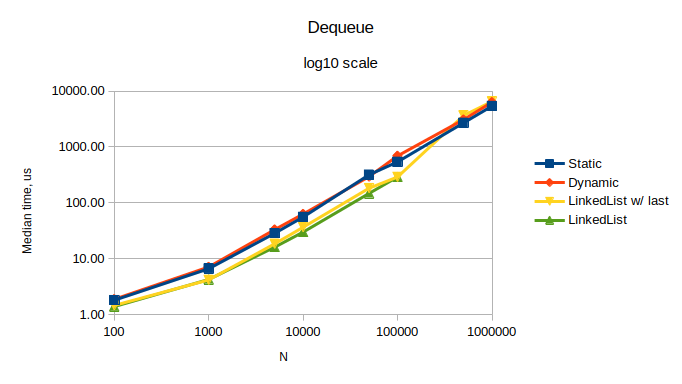
\includegraphics[width=\textwidth]{d.png}
        \caption{Median dequeue times}
        \label{fig:d}
    \end{figure}
\end{document}
